\textbf{3-1} 如力图3-1-1，劲度系数为 $k$ 的弹簧下端竖直悬挂着两个物体，质量分别为 $m_{1}$ 和 $m_2$。达到平衡后，突然撤去 $m_{2}$，试求 $m_{1}$ 运动的最大速度。

\begin{center}
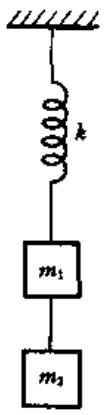
\includegraphics[width=0.05\textwidth]{figures/力图3-1-1.jpg}
\end{center}
\vfill

\textbf{3-2} 如力图3-2-1，水平弹簧一端固定，另一端系一质量为 $m$ 的小球，弹簧的劲度系数为 $k$，小球与水平面之间的摩擦系数为 $\mu$。当弹簧为原长时小球位于 O 点，开始时小球位于 O 点右方的 A 点，O 与 A 之间的距离为 $l_{0}$，从静止释放小球。

1. 为使小球能通过 O 点，而且只能通过 O 点一次，试问 $\mu$ 值应在什么范围？

2. 在上述条件下，小球在 O 点左方的停住点 B 点与 O 点的最大距离 $l_{1}$ 是多少？

\begin{center}
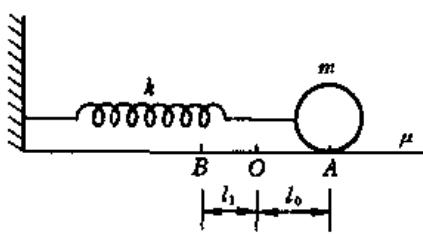
\includegraphics[width=0.25\textwidth]{figures/力图3-2-1.jpg}
\end{center}
\vfill

\newpage
\textbf{3-3} 如力图3-3-1所示，一木块沿倾角 $\theta = 30^{\circ}$ 的斜面从某初始位置以 $v_{0} = 4.5\,\mathrm{m/s}$ 的初速向上运动。已知木块与斜面之间的摩擦系数 $\mu = 0.35$。规定木块初始位置处的重力势能为零。试求木块动能等于重力势能处相对其初始位置的高度。
\begin{center}
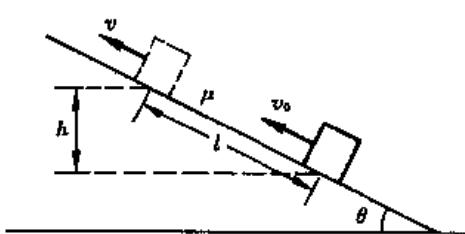
\includegraphics[width=0.15\textwidth]{figures/力图3-3-1.jpg}
\end{center}
\vfill

\textbf{3-4} 如力图3-4-1，在水平桌面上开有一孔，绳子的一部分平放在桌面上，另一部分经孔下垂。设绳不可伸长，均匀柔软，全长为 $l$，下垂长度为 $x_0$，从静止开始下落。设摩擦可略。试求在下落过程中，绳子速度随下落长度变化的规律，以及绳的下端位置随时间变化的规律。
\begin{center}
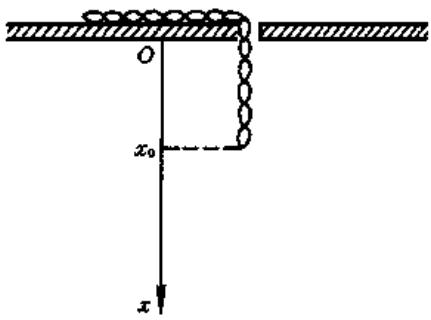
\includegraphics[width=0.15\textwidth]{figures/力图3-4-1.jpg}
\end{center}
\vfill

\newpage
\textbf{3-5} 如力图3-5-1，单摆的摆长为 $L$，摆球质量为 $m$，从左侧与竖直方向夹角 $\alpha$ 处静止下摆。在右侧，与悬点相距为 $r$、与竖直方向夹角为 $\beta$ $(\beta < \alpha)$ 处有一固定的钉子。设空气阻力可略。

试求：1. 为使小球能绕钉子作一个完整的圆周运动，角 $\alpha$ 至少应多大？2. 为使小球能与钉子相碰，角 $\alpha$ 应多大？

\begin{center}
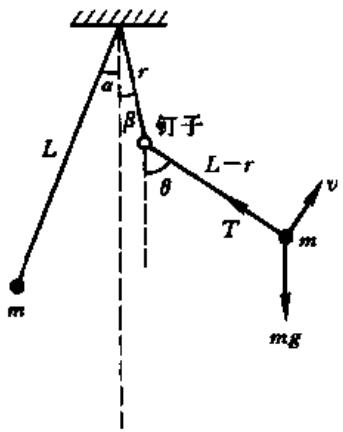
\includegraphics[width=0.2\textwidth]{figures/力图3-5-1.jpg}
\end{center}
\vfill

\textbf{3-6} 如力图3-6-1，质量为 $M$ 的圆环用细线（质量可略）悬挂，圆环上串着两个质量均为 $m$ 的小球，两小球自圆环顶端从静止开始同时向两边滑下，设摩擦可略。

\begin{center}
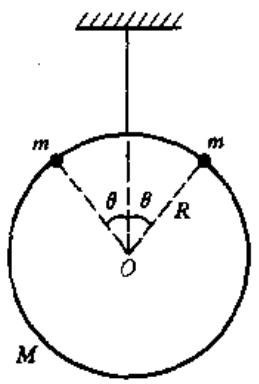
\includegraphics[width=0.15\textwidth]{figures/力图3-6-1.jpg}
\end{center}
\vfill

\newpage
\textbf{3-7} 如力图3-7-1，长为 $2r = 20\,\mathrm{cm}$、质量可以忽略的棒，中心点 $C$ 处有一固定的质量为 $m$ 的质点。棒一端 $A$ 点靠在竖直墙上，另一端 $B$ 点支在地面上，两端可分别沿墙和地面无摩擦地滑动。棒从竖直位置静止下滑，滑动过程中棒始终保持在同一竖直平面内。试求棒中心 $C$ 点触地的位置。

\begin{center}
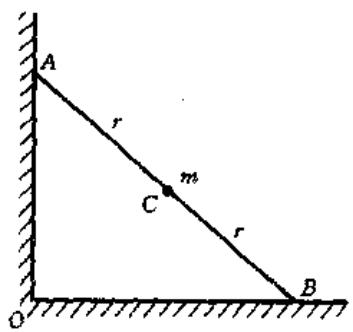
\includegraphics[width=0.2\textwidth]{figures/力图3-7-1.jpg}
\end{center}
\vfill

\textbf{3-8} 如力图3-8-1所示，长为 $L$ 的细杆顶端固定一小重球，竖直倒置在粗糙的水平地面上。小球处于不稳定的平衡状态，稍有扰动，小球将从静止开始向下跌落。假设细杆很轻，其质量可略。试求小球碰地时速度的水平分量和竖直分量。

\begin{center}
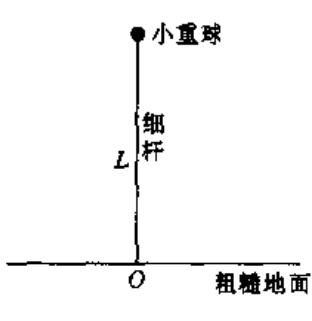
\includegraphics[width=0.2\textwidth]{figures/力图3-8-1.jpg}
\end{center}
\vfill

\newpage
\textbf{3-9} 如力图3-9-1，长为 $2l$ 的不可伸长的细绳一端固定于 $A$ 点的钉子上，另一端系一小球，小球可绕 $A$ 点在铅垂面内运动。开始时小球与 $A$ 点位于同一水平线上，小球在 $A$ 点右侧，垂直向下的初速度为 $v_{0}$。与 $A$ 点在同一水平线上左侧的 $B$ 点也有一钉子，$A$ 与 $B$ 之间的距离为 $l$。当细绳转到 $B$ 点后，小球将绕 $B$ 点向上运动。为使小球能与 $A$ 点的钉子相碰，试问小球初速 $v_{0}$ 的最小值应为多少？
\vfill

\textbf{3-10} 如力图3-10-1所示，在惯性系 $S$ 中有两质点 $A$ 和 $B$，质量分别为 $m_{1}$ 和 $m_{2}$，彼此间以万有引力相互吸引。开始时 $A$ 静止，$A$ 和 $B$ 相距 $l_{0}$，$B$ 以速度 $v_{0}$ 沿连线方向远离 $A$ 而运动 $(v_{0} < \sqrt{\frac{2Gm_2}{l_0}})$，$G$ 为引力常量。$B$ 受一指向其运动方向的变力 $F$ 的作用，使 $B$ 保持速度 $v_{0}$ 不变。

试求：1. 两质点之间的最大距离 $l_{\max}$。2. 从开始到最大距离过程中，变力 $F$ 所作的功（相对于惯性系 $S$）。

\begin{center}
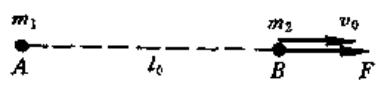
\includegraphics[width=0.3\textwidth]{figures/力图3-10-1.jpg}
\end{center}
\vfill

\newpage
\textbf{3-11} 如力图3-11-1，设想在地球表面的 $A$、$B$ 两地之间开凿一直通隧道，在 $A$ 处放置一小球，小球在地球引力的作用下从静止开始在隧道内运动。忽略一切摩擦阻力。试求小球的最大速度，以及小球从 $A$ 到 $B$ 所需的时间。已知地球半径为 $R$，地球表面的重力加速度为 $g$，$A$ 和 $B$ 之间的直线距离为 $L$。又设地球内部质量密度为恒量。

\begin{center}
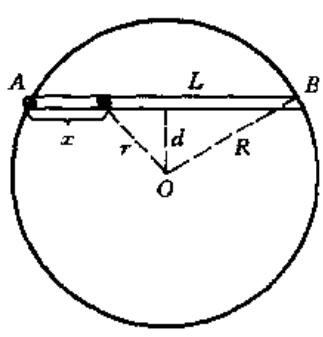
\includegraphics[width=0.2\textwidth]{figures/力图3-11-1.jpg}
\end{center}
\vfill

\textbf{3-12} 如力图3-12-1，两个质量均为 $m$ 的小球串在质量可忽略的光滑细杆上，用两根完全相同的弹簧相连，两弹簧的劲度系数均为 $k$，原长均为 $l_{0}$，左侧弹簧的左端固定在细杆的 $O$ 点，细杆绕 $O$ 点在水平面内转动。
\begin{center}
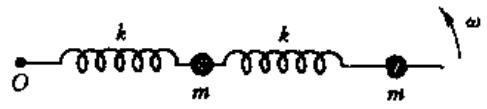
\includegraphics[width=0.15\textwidth]{figures/力图3-12-1.jpg}
\end{center}
\vfill

\newpage
\textbf{3-13} 如力图3-13-1，半径为 $R$ 的光滑圆环绕竖直的直径轴以角速度 $\omega$ 旋转。一质量为 $m$ 的小球串在圆环上，可沿环无摩擦地滑动。试求小球的平衡位置，并讨论平衡的稳定性。
\begin{center}
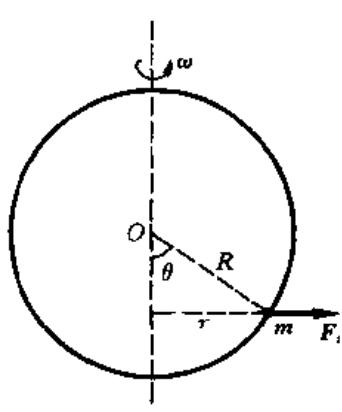
\includegraphics[width=0.15\textwidth]{figures/力图3-13-1.jpg}
\end{center}
\vfill

\textbf{3-14} 如力图3-14-1，在相距为 $l$ 的两平行弹性墙壁之间，有质量为 $m$ 的弹性小球以垂直于壁的初速度 $v_{0}$ 往返弹跳，设壁的质量远大于 $m$，碰撞是完全弹性的，重力及空气阻力可略。

试求：1. 每壁所受的平均作用力。2. 若用外力使左壁以速度 $V$ $(V \ll v_{0})$ 缓缓右移，证明外力作功等于小球动能的增加。
\begin{center}
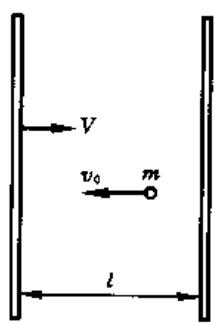
\includegraphics[width=0.15\textwidth]{figures/力图3-14-1.jpg}
\end{center}
\vfill

\newpage
\textbf{3-15} 如力图3-15-1，$A$、$B$、$C$ 三质点静止放置在光滑水平面上，它们的质量分别为 $m_{1}$、$m_{2}$、$m_{3}$，用柔软、不可伸长、质量可略的绳子相连并拉直，$AB$ 与 $BC$ 的夹角为 $\alpha$。以沿 $BC$ 方向的冲量 $I$ 作用于 $C$，试求质点 $A$ 开始运动时的初速。

\begin{center}
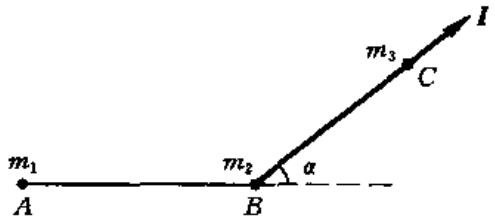
\includegraphics[width=0.2\textwidth]{figures/力图3-15-1.jpg}
\end{center}
\vfill

\textbf{3-16} 如力图3-16-1，从地面发射的炮弹在达到最高点处炸裂为质量相等的两块。第一块在炸裂后沿原方向运动，第二块则沿水平方向被弹出。已知炮弹发射的初速为 $v_0$，发射角为 $\theta$。忽略空气阻力，炸裂后第二块的落地点距发射点的水平距离为 $S_1$。试求第一块落地点距发射点的水平距离 $S_2$。

\begin{center}
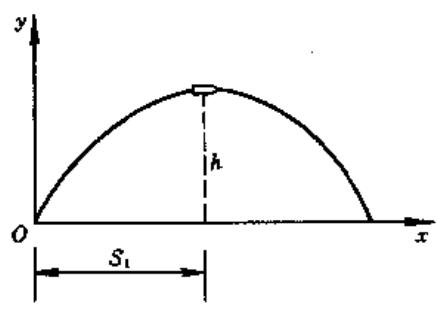
\includegraphics[width=0.2\textwidth]{figures/力图3-16-1.jpg}
\end{center}
\vfill

\newpage
\textbf{3-17} 地面上静止放置着质量为 $M$ 的平板车，车上有 $N$ 个人，每个人的质量均为 $m$。每个人以相同的相对速度 $u$（相对跳后的车速）沿水平方向从车后跳离平板车。忽略一切阻力。试问，在 $N$ 个人同时跳出和逐个跳出两种情况下，平板车在哪种情况下获得的动能大。
\vfill

\textbf{3-18} 如力图3-18-1，地面上有质量为 $M$、倾角为 $\theta$ 的斜面体，其顶端高 $h$ 处有质量为 $m$ 的小木块。开始时两者均静止，然后小木块从斜面体顶端滑至底部。忽略各种摩擦及阻力。试求：以地面为参考系，在小木块下滑过程中斜面体的支持力对它所作的功。

\begin{center}
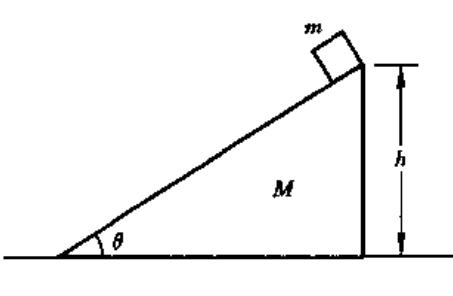
\includegraphics[width=0.2\textwidth]{figures/力图3-18-1.jpg}
\end{center}
\vfill

\newpage
\textbf{3-19} 如力图3-19-1，地面上静止地放置着质量为 $M$ 的木块，其底部为平面，上部有截面为半圆的凹槽，半径为 $R$，质量为 $m$ 的小球从最高处静止下滑。设各种摩擦及阻力均可略。试求：1. 在小球 $m$ 下滑过程中，$m$ 的绝对速度 $v$、$M$ 的绝对速度 $v_{M}$ 以及 $m$ 的相对速度 $v^{\prime}$ 随小球位置 $\theta$ 的变化规律。2. 小球 $m$ 在最低点时给木块 $M$ 的压力。

\begin{center}
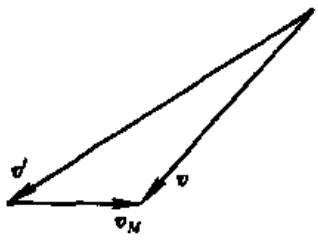
\includegraphics[width=0.2\textwidth]{figures/力图3-19-1.jpg}
\end{center}
\vfill

\textbf{3-20} 如力图3-20-1，质量为 $m_{3}$ 的木块平放在地面上，通过劲度系数为 $k$ 的竖直弹簧与质量为 $m_{2}$ 的木块相联，达到平衡。质量为 $m_{1}$ 的小球从距 $m_{2}$ 为 $h$ 的高处静止下落，与 $m_{2}$ 作完全非弹性碰撞。试问：为使 $m_{2}$ 向上反弹时能带动 $m_{3}$ 刚好离开地面，$h$ 应为多少？

\begin{center}
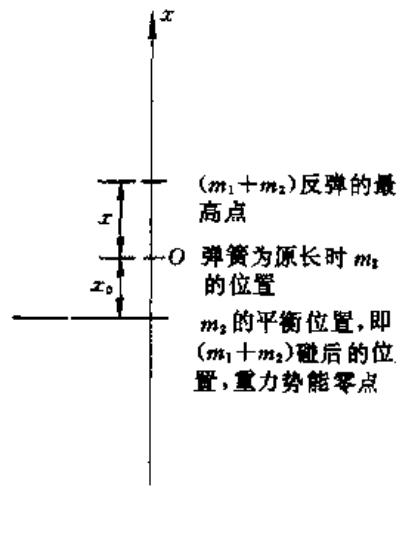
\includegraphics[width=0.25\textwidth]{figures/力图3-20-1.jpg}
\end{center}
\vfill

\newpage
\textbf{3-21} 如力图3-21-1所示，质量为 $M$ 的长滑块静止地放在光滑的水平桌面上，一质量可略的弹簧固定在滑块左端，弹簧的劲度系数为 $k$，滑块右端用一不可伸长的细绳固定在竖直墙上，细绳能承受的最大拉力为 $T_{0}$。一质量为 $m$，初速为 $v_{0}$（其方向水平向左）的小物在滑块上无摩擦地向左滑动，最终与弹簧相碰并压缩弹簧。
\begin{center}
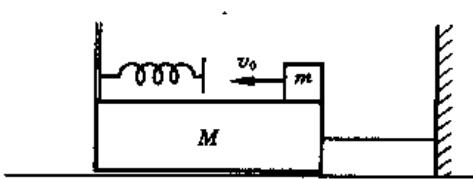
\includegraphics[width=0.2\textwidth]{figures/力图3-21-1.jpg}
\end{center}
\vfill

\textbf{3-22} 如力图3-22-1，球1和球2的质量分别为 $m_{1}$ 和 $m_{2}$，放置在光滑水平地面上，球1以一定的水平初速 $v_{10}$ 向右沿两球连心线运动，球2则静止。两球连心线右侧有一竖直弹性墙。设两球之间以及球与墙之间的所有碰撞均为完全弹性碰撞。为了使两球能发生、而且只能发生两次碰撞，试问两球的质量之比 $\dfrac{m_1}{m_2}$ 应满足什么条件？
\begin{center}
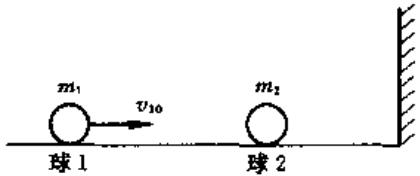
\includegraphics[width=0.2\textwidth]{figures/力图3-22-1.jpg}
\end{center}
\vfill

\newpage
\textbf{3-23} 如力图3-23-1，两根长度均为 $l$ 的刚性细杆，一端用质量为 $m$ 的球形铰链相连，两杆另一端分别安装质量为 $m$ 和 $2m$ 的小球。开始时两杆并拢，铰链球朝上，竖直放置在光滑桌面上，从静止释放，下面两球开始向两边滑动，两杆始终保持在同一铅垂面内。设三球本身的大小、轻杆的质量以及各种摩擦均可忽略。

\begin{center}
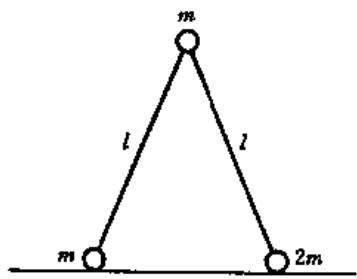
\includegraphics[width=0.2\textwidth]{figures/力图3-23-1.jpg}
\end{center}
\vfill

\textbf{3-24} 小球从高度为 $h$ 处静止下落，与地面碰撞时的恢复系数为 $e$。忽略空气阻力，忽略碰撞过程所需时间。
\vfill

\newpage
\textbf{3-25} 如力图3-25-1，台阶每级的宽和高均为 $l$。一小球向下逐级弹跳，每次反弹后，相对本级达到的最高高度均为 $H$，每次的下落点均在各级的同一地点。已知小球与台阶碰撞时的恢复系数为 $e$，忽略空气阻力。

\begin{center}
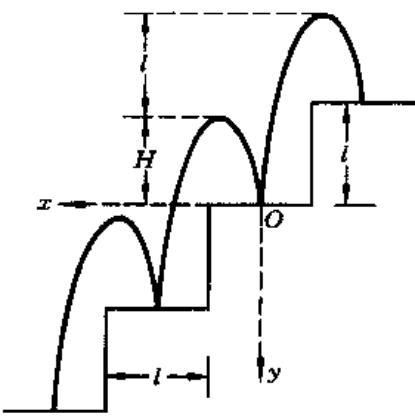
\includegraphics[width=0.2\textwidth]{figures/力图3-25-1.jpg}
\end{center}
\vfill

\textbf{3-26} 如力图3-26-1，在固定斜面的 $O$ 点上方 $h = 1.60\,\mathrm{m}$ 处有一小球从静止自由下落。已知斜面是光滑的，倾角为 $\theta = 15^{\circ}$，小球与斜面碰撞时的恢复系数为 $e = 0.60$，忽略空气阻力。

试求：1. 小球碰后达到的最高点与 O 点之间的高度差 $h_{\max}$。2. 设小球碰后落在斜面上 P 点，则 O 点与 P 点的距离 $S$ 是多少？3. 小球与斜面碰撞后，其机械能损失的百分数是多少？

\begin{center}
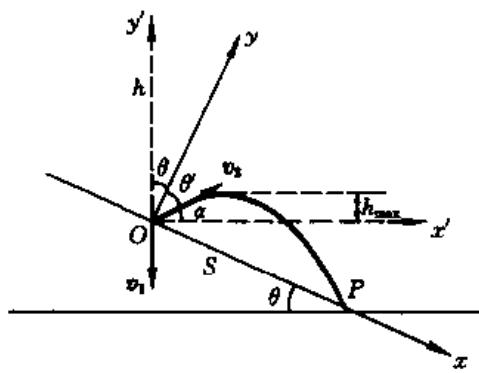
\includegraphics[width=0.3\textwidth]{figures/力图3-26-1.jpg}
\end{center}
\vfill

\newpage
\textbf{3-27} 如力图3-27-1，质量为 $M$ 的斜面体静止放置在光滑的水平桌面上，斜面体的倾角 $\theta = 15^{\circ}$。质量为 $m$ 的小球由静止自由下落到斜面体上，下落高度 $h = 1.60\,\mathrm{m}$。设斜面体表面是光滑的，并知小球碰后和碰前相对斜面体的相对速度在垂直于斜面方向的分量之比为 $e = 0.60$，碰撞点离桌面高度 $H = 1.00\,\mathrm{m}$，$M = 2m$。
\begin{center}
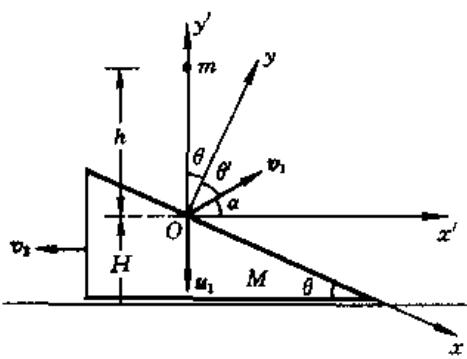
\includegraphics[width=0.2\textwidth]{figures/力图3-27-1.jpg}
\end{center}
\vfill

\textbf{3-28} 一平板放置在光滑水平桌面上，一小球在此桌面上运动并与平板作完全弹性碰撞，设小球也是光滑的。试证明：不论平板原来静止或处于运动状态，相对平板而言，小球总是遵守入射角等于反射角的规律。
\vfill

\newpage
\textbf{3-29} 如图3-29-1，均匀圆环静止放置在光滑水平桌面上，圆环质量为 $M$，半径为 $R$。一质量为 $m$ 的质点以速度 $v_0$ 沿圆环的直径方向射向圆环，碰撞是完全弹性的。试求碰后圆环的运动状态和质点的运动状态。
\begin{center}
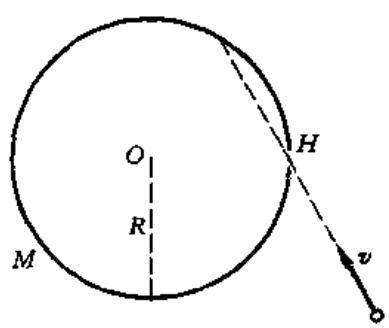
\includegraphics[width=0.2\textwidth]{figures/图3-29-1.jpg}
\end{center}
\vfill

\textbf{3-30} 三质点的质量分别为 $m_{1}$、$m_{2}$、$m_{3}$，以万有引力相互作用，绕垂直于三质点所在平面并通过质心 C 的转轴旋转。

试问：为使三质点的相对位置保持不变，需满足什么条件？
\vfill

\newpage
\textbf{3-31} 质量为 $M$ 的平板车静止在光滑地面上，车上有 $N$ 个人，每人的质量均为 $m$，若每人消耗同样的体力（即每人作功相同）沿水平方向向后跳，忽略空气阻力，人可看作是质点。
\vfill

\textbf{3-32} 如力图3-32-1，质量分别为 $m_{1}$ 和 $m_{2}$ 的两木块用劲度系数为 $k$ 的弹簧相连，静止地放在光滑地面上。质量为 $m$ 的子弹以水平初速 $v_{0}$ 射入木块 $m_{1}$，设子弹射入过程的时间极短。
\begin{center}
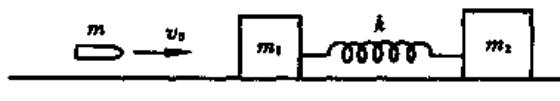
\includegraphics[width=0.2\textwidth]{figures/力图3-32-1.jpg}
\end{center}
\vfill

\newpage
\textbf{3-33} 如力图3-33-1，在光滑地面上静止地放着质量为 $m$ 的箱子。在箱内光滑的底面上，质量也为 $m$ 的滑块以水平初速 $v_{0}$ 开始运动，并与两壁反复碰撞。已知滑块与箱子每碰一次后，两者的相对速度改变 $e = \sqrt[4]{\frac{1}{2}}$ 倍。

试求：1. 最多经几次碰撞后，系统总能量的损耗不大于40\%。2. 从滑块开始运动到完成上述次数的碰撞后，箱子的平均速度是多少？
\begin{center}
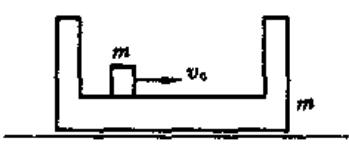
\includegraphics[width=0.2\textwidth]{figures/力图3-33-1.jpg}
\end{center}
\vfill

\textbf{3-34} 动能为 $E_0$ 的 ${}^4\mathrm{He}$ 核轰击静止的 ${}^7\mathrm{Li}$ 核，作完全非弹性碰撞后成为复合核 ${}^{11}\mathrm{B}$，${}^{11}\mathrm{B}$ 进一步分裂为 ${}^{10}\mathrm{B}$ 和中子 ${}^1\mathrm{n}$。上述核反应过程需消耗能量 $Q = 2.8\,\mathrm{MeV}$。反应方程为
\[
{}^4\mathrm{He} + {}^{7}\mathrm{Li} \rightarrow ({}^{11}\mathrm{B}) \rightarrow {}^{10}\mathrm{B} + {}^{1}\mathrm{n} - 2.8\,\mathrm{MeV}
\]

试求：上述核反应过程所需的 $E_{0}$ 的最小值是多少？相应的中子动能为多大？
\vfill

\newpage
\textbf{3-35} 一物体作直线运动，其质量不断随时间变化。设该物体在 $t$ 时刻的质量为 $M(t)$，速度为 $v(t)$。试证明下述密舍尔斯基方程：
\[
M\frac{\mathrm{d}v}{\mathrm{d}t} = (u - v)\frac{\mathrm{d}M}{\mathrm{d}t} + F
\]

式中 $F$ 是质量不断变化的主体所受的合外力，$u$ 是附加物附加到主体前的绝对速度或抛出物抛离主体后的绝对速度。
\vfill

\textbf{3-36} 竖直下垂的绳子从静止自由下落，开始时绳下端刚好与地面接触。设绳均匀柔软，全长为 $l$。

试证明：下落过程中地面所受压力等于已经落在地面上的绳子重量的3倍。
\vfill

\newpage
\textbf{3-37} 火箭从地面竖直向上发射。已知火箭自身质量为 $M_{s}$，燃料的初始质量为 $M_{f}$，燃气相对火箭的喷射速度为 $v^{\prime}$，单位时间的喷气质量为 $a$。设在火箭上升的高度范围内 $g$ 为常量，忽略空气阻力。

试求：1. 火箭的推力和加速度。2. 任意时刻火箭的速度和上升高度。3. 燃料耗尽时，火箭的加速度、速度和高度。4. 火箭能达到的最大高度及所需时间。
\vfill

\textbf{3-38} 如力图3-38-1，质量为 $m$ 的小球下系一条足够长的柔软均匀且不可伸长的绳子。绳子的质量线密度为 $\lambda$。将小球以初速 $v_{0}$ 从地面竖直上抛，忽略空气阻力。

试问：在上升过程中，小球的速率怎样随高度变化？
\begin{center}
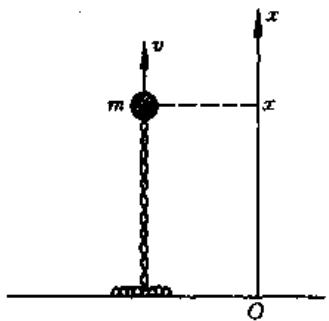
\includegraphics[width=0.25\textwidth]{figures/力图3-38-1.jpg}
\end{center}
\vfill

\newpage
\textbf{3-39} 球状小水滴在静止的雾气中下落，下落过程中吸附了全部所遇到的水分子。设水滴始终保持球状，设雾气密度均匀，忽略空气的粘滞力，重力加速度取恒定值 $g$。

试证明经过足够长时间后，水滴加速度趋于稳定值，并求出此稳定值。
\vfill
